%Paul E. West

%\documentclass[xcolor=svgnames]{beamer}
\documentclass{beamer}
\usepackage[boxed,vlined,figure]{algorithm2e}

%\usecolortheme[named=FireBrick]{structure}
%\usecolortheme[named=black]{structure}
%\usecolortheme{beetle}
%\usecolortheme{beaver}
%\usecolortheme{crane}
%\usecolortheme{dolphin}
%\usecolortheme{dove}
%\usecolortheme{fly}
%\usecolortheme{lily}
\usecolortheme{orchid}
%\usecolortheme{rose}
%\setbeamercolor{background canvas}{bg=Gold!25}
%\setbeamercolor{background canvas}{bg=Black!100}
%\setbeamercolor{foreground}{bg=Gold!25}
%\setbeamercolor{normal text}{fg=green,bg=black}
%\setbeamercolor*{palette primary}{use=structure,fg=green,bg=black}

\mode<presentation>{
    \usetheme{Darmstadt}
    \setbeamercovered{invisible}
    %\setbeamercovered{transparent}
    \setbeamercolor*{palette primary}{use=structure,fg=white,bg=blue}
    \setbeamercolor*{palette secondary}{use=structure,fg=white,bg=blue}
    \setbeamercolor*{palette tertiary}{use=structure,fg=white,bg=blue}
}

\usepackage[english]{babel}
\usepackage[latin1]{inputenc}
\usepackage{times}
\usepackage[T1]{fontenc}
%\usepackage{epsfig}
\usepackage{ulem}
\usepackage{color,soul}

\usepackage{graphicx}
\usepackage{amssymb}
\usepackage{url,hyperref}
\definecolor{beamer@blendedblue}{rgb}{1,.6,.2}
%\usepackage{tikz}
%\usetikzlibrary{shapes}
%\usetikzlibrary{arrows}
%\tikzstyle{block}=[draw opacity=0.7, line width=1.4cm]
\usepackage{listings}
\lstset{language=C}
\lstset{tabsize=4}
\lstset{basicstyle=\tiny}


%\usecolortheme[overlystylish]{albatross}
%\usecolortheme[]{lily}
%\usecolortheme[]{albatross}
%\usecolortheme[]{orchid}
%\setbeamercolor{normal text}{fg=green!10}

\title{COIN 330: Computer Architecture}
\author{Dr. Paul E. West}

\institute{
  Department of Computer Science\\
  Charleston Southern University
}

\date{January 15, 2015}

\subject{Computer Architecture}
%\keywords{Performance Counters, Multicore}

%\pgfdeclareimage[height=1.0cm]{university-logo}{../imgs/csu-logo}
\pgfdeclareimage[height=0.75cm]{university-logo}{../imgs/csu-logo}
%\pgfdeclareimage[height=0.50cm]{university-logo}{../imgs/csu-logo}
\logo{\pgfuseimage{university-logo}}

\begin{document}

\begin{frame}
  \titlepage
\end{frame}

\section{First Day}
\subsection{}
\begin{frame}{About the Professor}
\begin{itemize}
\item PhD from Florida State University in Computer Science
\begin{itemize}
\item College of Charleston: Adjunct 2013-2014
\end{itemize}
\item Work Experience:
\begin{itemize}
\item Google (2014): Android Bluetooth/Wi-Fi/Telephony
\item SPAWAR (2009-2014): Communication systems
\item DenimGroup (2004-2005): Start-up; web design and network security
\end{itemize}
\end{itemize}
\end{frame}

\begin{frame}{Syllabus}
Lets go over the syllabus...
\end{frame}

\begin{frame}{Complex Yet Simple}
\begin{itemize}
\item Computers are some of the more complex devices humans have created.
\item Yet, are simple in many ways.  EX:
\begin{itemize}
\item A CPU (where a lot of the ``work'' occurs) is basically a bunch of transistors etched on silicon.
\item `a bunch' can be $>$ billions
\end{itemize}
\end{itemize}
\end{frame}

\begin{frame}{From C to Execution}
\begin{itemize}
\item How does the code that you type in go from text to executing on the computer?
\item How does a piece of silicon turn you ``English-like'' C code into a dynamic computation?
\item We will explore these in more depth.
\end{itemize}
\end{frame}

\begin{frame}{Logic}
\begin{itemize}
\item The computer executes your program (set of instructions) through electronic signals.
\item These signals (in general) are executed in steps (clock cycle).
\item Our job here is to see how this is done and give you an idea of how a computer can be built to do computations.
\end{itemize}
\end{frame}

\section{State of Computers}
\subsection{}
\begin{frame}{The Computer Revolution}
\begin{itemize}
\item Progress in computer technology
\begin{itemize}
\item Underpinned by Moore's Law 
\end{itemize}
\item Makes novel applications feasible
\begin{itemize}
\item Computers in automobiles
\item Cell phones
\item Human genome project
\item World Wide Web
\item Search Engines
\end{itemize}
\item Computers are pervasive
\end{itemize}
\end{frame}

\begin{frame}{Classes of Computers}
\begin{itemize}
\item Personal computers
\begin{itemize}
\item General purpose, variety of software
\item Subject to unit cost vs performance tradeoff
\end{itemize}
\item Server computers
\begin{itemize}
\item Network based
\item High capacity, performance, reliability
\item Range from small servers to building sized
\end{itemize}
\end{itemize}
\end{frame}

\begin{frame}{Classes of Computers}
\begin{itemize}
\item Supercomputers
\begin{itemize}
\item High-end scientific and engineering calculations
\item Highest capability but represent a small fraction of the overall computer market 
\item \url{http://www.top500.org} maintains a list
\end{itemize}
\item Embedded computers
\begin{itemize}
\item Hidden as components of systems
\item Stringent power/performance/cost constraints
\end{itemize}
\end{itemize}
\end{frame}

\subsection{}
\begin{frame}{The PostPC Era}
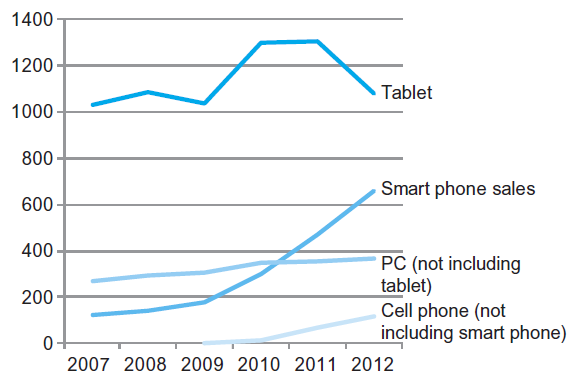
\includegraphics[width=1.0\textwidth]{../imgs/post-pc-era.png}
\end{frame}

\begin{frame}{The PostPC Era}
\begin{itemize}
\item Personal Mobile Device (PMD)
\begin{itemize}
\item Battery operated
\item Connects to the Internet
\item Hundreds of dollars
\item Smart phones, tablets, electronic glasses, smart watches
\end{itemize}
\item Cloud computing
\begin{itemize}
\item Warehouse Scale Computers (WSC)
\item Software as a Service (SaaS)
\item Portion of software run on a PMD and a portion run in the Cloud
\item Amazon and Google
\end{itemize}
\end{itemize}
\end{frame}

\section{Conclusion}
\subsection{}
\begin{frame}{What you Will Learn}
\begin{itemize}
\item How programs are translated into the machine language
\item And how the hardware executes them
\item The hardware/software interface
\item What determines program performance
\item And how it can be improved
\item How hardware designers improve performance
\item What is parallel processing
\end{itemize}
\end{frame}

%\begin{frame}{Event Based Processor}
%\begin{columns}[c]
%\column{0.25\textwidth}
%\begin{block}{OS driven Execution}
    %\includegraphics[width=1.0\textwidth]{diagrams/normproc.png}
%\end{block}
%\column{0.25\textwidth}
%\begin{block}{Event Driven Execution}
    %\includegraphics[width=1.0\textwidth]{diagrams/eventproc.png}
%\end{block}
%\column{0.5\textwidth}
%\begin{itemize}
    %\item Normal execution: kernel/software driven
    %\item Event based : event driven
    %\item Performance monitoring is event based
    %\item Next task based on event not scheduled by kernel
    %\item 5.92 times speedup for control dominated programs
%\end{itemize}
%\end{columns}
%\end{frame}

\end{document}
